\documentclass[hidelinks,12pt]{article}

\usepackage{amsmath}    % need for subequations
\usepackage{graphicx}   % need for figures
\usepackage{verbatim}   % useful for program listings
\usepackage{color}      % use if color is used in text
\usepackage{subfigure}  % use for side-by-side figures
\usepackage{hyperref}   % use for hypertext links, including those to external documents and URLs

\usepackage[numbered]{matlab-prettifier} % including matlab w/ syntax highlighting
\usepackage[T1]{fontenc} % prettier matlab font
\lstMakeShortInline[style=Matlab-editor]| % matlab inline escape character

\usepackage[
top    = 2.75cm,
bottom = 2.50cm,
left   = 3.00cm,
right  = 2.50cm]{geometry}

\graphicspath{ {./Figures/} }

% don't need the following. simply use defaults
\setlength{\baselineskip}{16.0pt}    % 16 pt usual spacing between lines



\begin{document}
\pagenumbering{gobble}
\begin{center}
  {\huge Homework 5}\\
  \vspace{10px}
  
\includegraphics{Logo} \\
  Date of Submission:\\
  February 25, 2019\\
  \vspace{30px}
  \rule{300px}{0.5px} \\
  Thorne Wolfenbarger \\
  \href{mailto:wolfent1@my.erau.edu}{wolfent1@my.erau.edu} \\
  \vspace{30px}
  Submitted to: \\
  Professor Kaela Martin \\
  College of Engineering \\
  \vspace{40px}
  In Partial Fulfillment \\
  of the Requirements of \\
  \vspace{10px}
  AE 313 \\
  Space Mechanics \\
  Spring, 2019 \\
\end{center}

\pagenumbering{arabic}
\begin{center}
\large AE 313 Homework 7
\end{center}
\flushleft
1. What is the initial Jason orbit semi-major axis, eccentricity, and true anomaly?\\
\begin{lstlisting}[frame=lines,style=Matlab-editor,basicstyle = \mlttfamily]
syms am
eq = -MU/(2*am) == vm^2/2 - MU/rm;
am = double(solve(eq, am)) % 6.6993e3 km

hm = rm*vm*cosd(FPAm);
pm = hm^2/MU;
em = sqrt(1-pm/am) % 0.5001

true_am = atan2d(rm*vm^2/MU*cosd(FPAm)*sind(FPAm),rm*vm^2/MU*cosd(FPAm)^2-1) % 160.0052
\end{lstlisting}
\begin{tabular}{rl}
  $a^-=$&6699.3~km\\
  $e^-=$&0.5001$^\circ$\\
  $\theta^{*-}=$&160.0052$^\circ$
\end{tabular}\\
\vspace{10px}
2. Draw the vector diagram.\\
~On a separate page\\
\vspace{10px}
3. Determine the velocity and flight path angle immediately following the
maneuver. Make sure to justify if $\Delta \gamma$ is positive or negative.\\
\begin{lstlisting}[frame=lines,style=Matlab-editor,basicstyle = \mlttfamily]
syms vp FPAp
vp = sqrt(vm^2 + dv^2 - 2*vm*dv*cosd(180 - abs(alpha))) % 6.1136 km/s
dFPA = acosd(((dv^2)-(vm^2)-(vp^2))/(-2*vm*vp)) %11.5652 deg | negative because the dv is oriented towards earth (indicated by the negative alpha)
FPAp = FPAm - dFPA;
\end{lstlisting}
\begin{tabular}{rl}
  $v^+=$&6.1136~km/s\\
  $\gamma^+=$&6.3148$^\circ$\\
\end{tabular}\\
$\Delta \gamma$ is negative because $\lvert \Delta \vec{v} \rvert$ is oriented towards earth (indicated by the negative alpha).\\
\newpage
4. Determine the orbital characteristics following the maneuver: $a^+, e^+, \theta^{*+}, \Delta \omega$\\
\begin{lstlisting}[frame=lines,style=Matlab-editor,basicstyle = \mlttfamily]
FPAp = FPAm - dFPA;
syms ap
rp = rm;
eq = -MU/(2*ap) == vp^2/2 - MU/rp;
ap = double(solve(eq, ap)) % 8.5290e+03 km
ep = sqrt((rp*vp^2/MU - 1)^2*cosd(FPAp)^2 + sind(FPAp)^2) % 0.1560
true_ap = atan2d(rp*vp^2/MU*cosd(FPAp)*sind(FPAp),rp*vp^2/MU*cosd(FPAp)^2 - 1)
true_ap = atan2d(rp*vp^2/MU*cosd(FPAp)*sind(FPAp),rp*vp^2/MU*cosd(FPAp)^2-1); % 141.4710
dAOP = -(true_ap - true_am) % 18.5342
\end{lstlisting}
\begin{tabular}{rl}
$a^+=$&8529~km\\
$e^+=$&0.1260\\
$\theta^{*+}=$&141.71$^\circ$\\
$\Delta \omega=$&18.5342$^\circ$\\
\end{tabular}
$\theta^{*+}$'s value is positive due to the fact that $atan2$ takes into account the signs of the components. $\Delta \omega=$18.5342$^\circ$ is a positive value due to the fact that it follow's the relationship of $\Delta \omega = \theta^{*-} - \theta^{*+}$.
\newpage
5. Use GMAT to plot the two orbits. Propagate both orbits at least one
period. Draw the vector diagram (vm, vp, alpha, dFPA, dv) and position
vector for the maneuver on the printout. Check $a^+, e^+, \theta^*, v^+$.
\begin{figure}[!htb]
  \center
  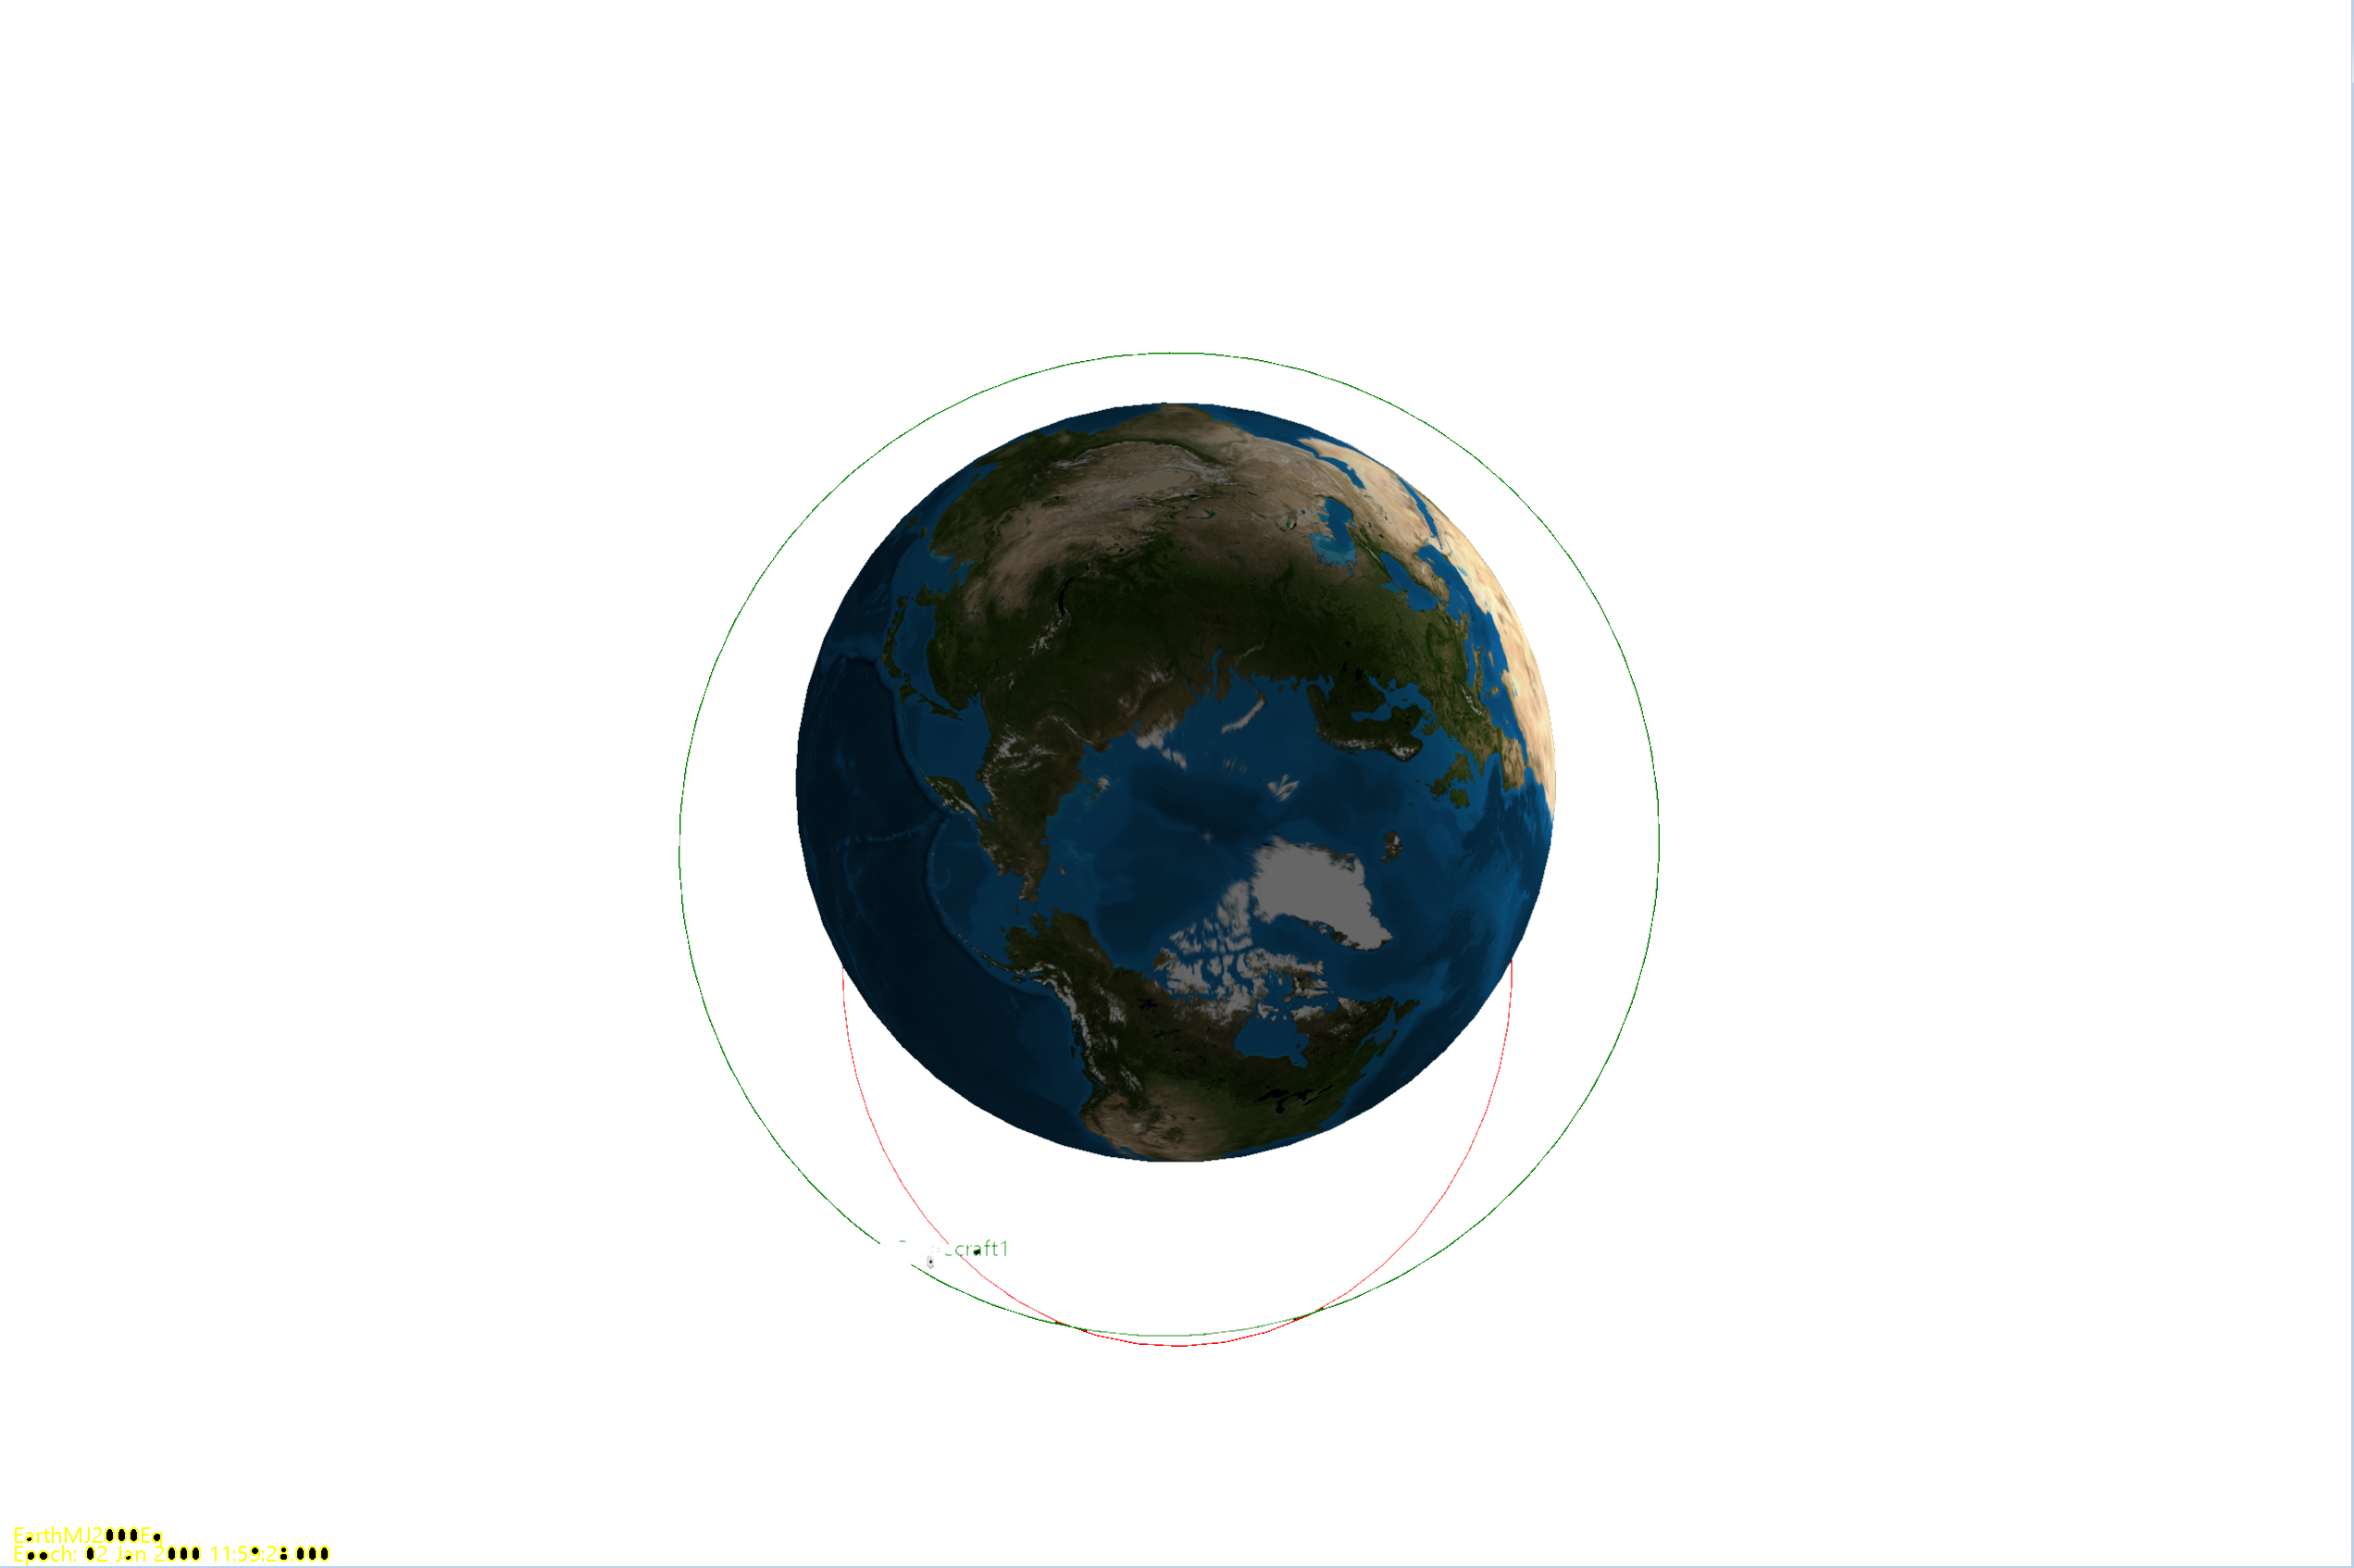
\includegraphics[scale=0.23]{Orbits}
  \caption{GMAT Plot of Orbits}
  \label{fig:GMAT}
\end{figure}\\
\begin{tabular}{rl}
$a^+=$&8529~km\\
$e^+=$&0.1560\\
$\theta^{*+}=$&141.471$^\circ$\\
$v^+=$&6.1136~km/s\\
\end{tabular}\\
\vspace{5px}
6. What would happen if you failed to perform this maneuver?\\
~Without the maneuver, ICESAT-2 is on a parabollic collision trajectory with Earth. If the maneuver failed, the spacecraft would crash into Earth. This can be observed in (Fig. \ref{fig:GMAT}) where the smaller, red orbit displays the collision trajectory.
\newpage
HW5.m
\begin{lstlisting}[frame=lines,style=Matlab-editor,basicstyle = \mlttfamily]
clc; clear all; close all

%constants
MU = 42828;

% Problem 1
vr = [-2089.6 -2515.7 -6382.0];
vv = [2.1744 0.76911 0.13452];

r = norm(vr)
v = norm(vv)

vh = cross(vr, vv);
h = norm(vh);

syms a
energy_eqn = v^2/2 - MU/r == -MU/(2*a)
energy = v^2/2 - MU/r
a = double(solve(energy_eqn, a))

syms e
h_eqn = h == sqrt(MU*a*(1-e^2))
e = double(solve(h_eqn,e))
e = max(e)

syms E
E_eqn = r == a*(1-e*cos(E));
E = double(solve(E_eqn,E));
E = -min(E) %Because it is descending.

syms time_since_p
time_since_p_eqn = sqrt(MU/a^3)*time_since_p == E - e*sin(E);
time_since_p = double(solve(time_since_p_eqn,time_since_p))

% Problem 2
p = h^2/MU;
true_a = -acos(p/(r*e) - 1/e)
vv_rt = [h*e/p*sin(true_a) h/r 0] % answer

% Problem 3
E1 = E;
t1 = time_since_p;
vr1 = vr;
vv1 = vv;
r1 = r;
v1 = v;
t2 = time_since_p + 12*60*60;
n = sqrt(MU/a^3);
M = n*t2;
E2 = fzero(@(x) x-e*sin(x)-M, 0);
f = 1 - a/r*(1-cos(E2-E1));
g = (t2 - t1) - sqrt(a^3/MU)*(E2 - E1 - sin(E2 - E1));

vr2 = f*vr + g*vv;
r2 = norm(vr2);
fdot = -sqrt(MU*a)/(r2*r1)*sin(E2-E1);
gdot = 1 - a/r2*(1-cos(E2-E1));

vv2 = fdot*vr1 + gdot*vv1 % intertial unit vectors

true_a2 = -acos(p/(r2*e) - 1/e)

vv2_rt = [h*e/p*sin(true_a2) h/r2 0] % radial-tangential

% Problem 4
vr2_peri = [r2*cos(true_a2) r2*sin(true_a2) 0]
vv2_peri = sqrt(MU/p)*[-sin(true_a2) e+cos(true_a2) 0]

% Problem 5

% find i theta omega
syms inc
h_hat = cross(vr2, vv2)/norm(cross(vr2, vv2))
inc_eqn = cos(inc) == dot(h_hat, [0 0 1])
inc = double(solve(inc_eqn,inc))
inc = max(inc)

syms RAAN
RAAN_eqn_1 = sin(RAAN)*sin(inc) == dot(h_hat, [1 0 0])
RAAN_eqn_2 = -cos(RAAN)*sin(inc) == dot(h_hat, [0 1 0])
RAAN1 = double(solve(RAAN_eqn_1));
RAAN2 = double(solve(RAAN_eqn_2));
RAAN = min(RAAN1)*180/pi

syms arg_peri
r1_hat = vr1/norm(vr1)
theta_hat = cross(r1_hat, h_hat)/norm(cross(r1_hat, h_hat))
syms theta
theta_eqn_1 = sin(inc) * sin(theta) == dot(r1_hat, [0 0 1])
theta_eqn_2 = sin(inc) * cos(theta) == dot(theta_hat, [0 0 1])
theta1 = double(solve(theta_eqn_1, theta))
theta2 = double(solve(theta_eqn_2, theta))
theta = intersect(theta1, theta2)
arg_peri_eqn = arg_peri == theta - true_a
arg_peri = double(solve(arg_peri_eqn, arg_peri))
\end{lstlisting}

\end{document}
